\chapter{微分積分の発展}\label{chapt:calculus_app}

\section{テーラー展開}

\pref{eq:linear_approx00}で学んだ線型近似は, 関数を一次式(直線の式)で近似する考え方である。
ところが, 本来, 一次式より二次式や
三次式のほうが多様な関数を表現できるので, 関数を二次式や三次式, いや, もっとたくさんの次数の
多項式で近似するほうが, 高い精度が得られるだろう。次数を無限大にすれば, もとの関数と近似式の
間の誤差を限りなく0にすることもできるかも! そうだったら素敵だ! 多項式は四則演算(加減乗除)だけで計算でき, 
微分も積分も簡単だから, 取り扱いが楽だし。そこで, 以下のように関数$f(x)$を多項式で近似することを考えよう:
\begin{eqnarray}f(x)=a_0+a_1x+a_2x^2+\cdots+a_nx^n+\cdots\nonumber\\\label{eq:Taylor0}\end{eqnarray}
この左辺と右辺が一致するなら, それぞれを$x=0$において何回か微分したもの
($x=0$での微分係数)も等しいはずなので, 
\begin{eqnarray*}
f(0)&=&a_0\\
f'(0)&=&a_1\times1\\
f''(0)&=&a_2\times1\times2\\
f'''(0)&=&a_3\times1\times2\times3\\
&&\cdots\\
f^{(n)}(0)&=&a_n\times1\times2\times3\cdots\times n
\end{eqnarray*}
となるはずだ。ここで, $f^{(n)}(x)$は, $f(x)$の$n$階導関数である。
$(x^n)$を$n$回微分すると$1\times2\times3\cdots\times n=n!$となることに注意せよ。すると, 
\begin{eqnarray*}
a_0&=&f(0)\\
a_1&=&f'(0)/1\\
a_2&=&f''(0)/(1\times2)\\
a_3&=&f'''(0)/(1\times2\times3)\\
&&\cdots\\
a_n&=&f^{(n)}(0)/n!
\end{eqnarray*}
となることがわかる。すなわち, \eref{eq:Taylor0}は, 次式のようになる
\footnote{$0!$は$1$とする。}:
%\begin{itembox}{マクローリン展開}
\begin{eqnarray}
f(x)&=& \frac{f(0)}{0!}+\frac{f'(0)}{1!} x+\frac{f''(0)}{2!} x^2+\cdots\nonumber\\
&=&\sum^{\infty}_{n=0} \frac{f^{(n)}(0)}{n!}x^n\label{eq:macl}
\end{eqnarray}
%\end{itembox}
これを, 関数$f(x)$の\underline{マクローリン展開} \index{まくろーりんてんかい@マクローリン展開}という。


\begin{q}\label{eq:Maclaurin_linear_approx} \eref{eq:macl}は
\pref{eq:linear_approx00}の\eref{eq:linear_approx00}で出てきた線型近似の式
\begin{eqnarray*}
f(x) \fallingdotseq f(0)+f'(0)x
\end{eqnarray*}
の拡張になっていることを説明せよ。\end{q}


ここまでは$x=0$での微分係数を考えたが, 一般に, $x=a$での微分係数を考えると, 
%\begin{itembox}{テーラー展開}
\begin{eqnarray}
f(x)&=& \frac{f(a)}{0!}+\frac{f'(a)}{1!} (x-a)+\frac{f''(a)}{2!} (x-a)^2+\cdots\nonumber\\
&=&\sum^{\infty}_{n=0} \frac{f^{(n)}(a)}{n!}(x-a)^n \label{eq:Taylor_expansion}
\end{eqnarray}
%\end{itembox}
となる。これを関数$f(x)$の$x=a$のまわりでの\underline{テーラー展開} \index{てーらーてんかい@テーラー展開}という
\footnote{ただし, テーラー展開できない関数もある。また, 特定の定義域($x$の取りうる値の範囲)
でしかテーラー展開できない場合もある。どのような関数が, どのような定義域でテーラー展開
できるのか, ということは, 大学の数学の教科書を参照せよ。}。\\

マクローリン展開は, テーラー展開の一種である。$x=0$のまわりのテーラー展開がマクローリン展開である。
しかし, 世間的にはテーラー展開と言えば, マクローリン展開のことを意味することも多い。\\

ところで, 導関数の定義\eref{eq:define_dif}(P.\pageref{eq:define_dif})において, $x_0$を$a$と書き換えれば, 
\begin{eqnarray}
f(a+dx)=f(a)+f'(a) dx
\end{eqnarray}
となる。さらに, $a+dx$を改めて$x$と書き換えれば, $dx=x-a$となり, この式は, 
\begin{eqnarray}
f(x)=f(a)+f'(a) (x-a)
\end{eqnarray}
となる。これは, 線型近似の式であり, テーラー展開の式の最初の2項と一致する。
ただしこの式は, $x-a$, つまり$dx$が十分に0に近いときにしか成り立たない。
従って, テーラー展開の式は, 導関数の定義式(あるいは線型近似)を, $dx$が0に近くなくても
成り立つように, 拡張したものだ, とも言える。

\begin{q}\label{q:univ_Taylor0} $e^x$, $\sin x$, $\cos x$をそれぞれ
マクローリン展開 ($x=0$のまわりでテーラー展開)すると, 以下の式になることを示せ:
\begin{eqnarray}
&&e^x = \frac{1}{0!}+\frac{x}{1!}+\frac{x^2}{2!}+\frac{x^3}{3!}+\frac{x^4}{4!}+\cdots\label{eq:Taylor_exp0}\\
&&\sin x = \frac{x}{1!}-\frac{x^3}{3!}+\frac{x^5}{5!}-\frac{x^7}{7!}+\cdots\label{eq:Taylor_sin0}\\
&&\cos x=\frac{1}{0!}-\frac{x^2}{2!}+\frac{x^4}{4!}-\frac{x^6}{6!}+\cdots\label{eq:Taylor_cos0}
\end{eqnarray}\end{q}
\vspace{0.3cm}

\begin{figure}[h]
    \centering
    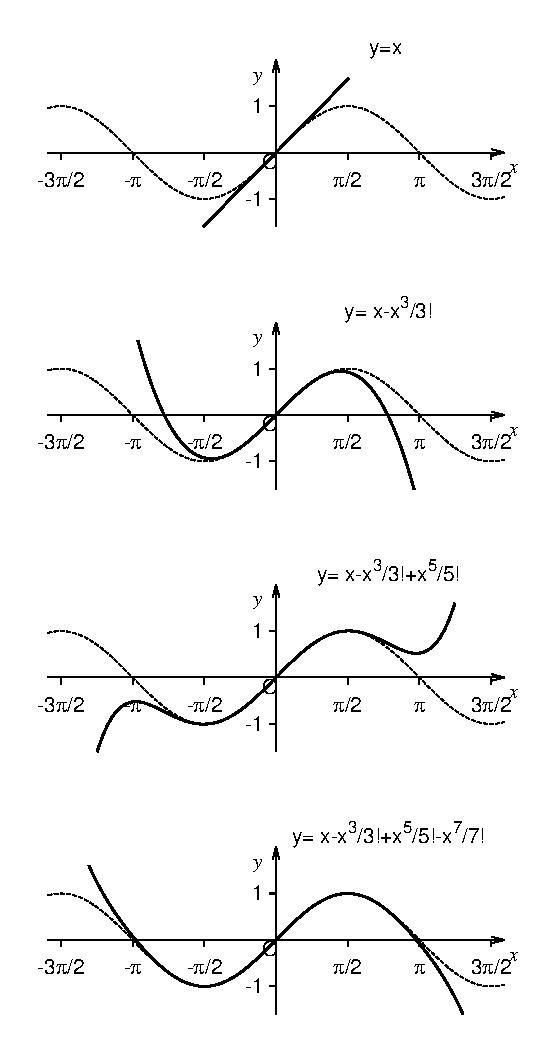
\includegraphics[width=8cm]{Taylor_sin.eps}
    \caption{実線は$y=\sin x$のマクローリン展開 (1次, 3次, 5次, 7次近似)。点線は$y=\sin x$}
\end{figure}

\begin{q}\label{q:univ_Taylor2} $e^x$, $\sin x$, $\cos x$のそれぞれのマクローリン展開
($x=0$のまわりでのテーラー展開)の式を用いて, 
\begin{eqnarray*}
&&(e^x)'=e^x\\
&&(\sin x)'=\cos x\\
&&(\cos x)'=-\sin x
\end{eqnarray*}
を確認せよ。
\end{q}\vspace{0.3cm}

\begin{q}\label{q:Taylor_Napier} \eref{eq:Taylor_exp0}から, 次式を導け:
\begin{eqnarray}
e=\frac{1}{0!}+\frac{1}{1!}+\frac{1}{2!}+\frac{1}{3!}+\cdots+\frac{1}{n!}+\cdots\label{q:compute_Napier_again}
\end{eqnarray}
これは, \pref{exmpl:compute_Napier}の例\ref{exmpl:compute_Napier}で
コンピュータが出した結果を理論的に裏付けるものである。\end{q}\mv


\begin{faq}{\small \textgt{なぜ近似する必要があるのですか。2次近似, 3次近似, ...と, 
どんどん近づけたら元の関数にものすごく近くなって近似する意味がよくわかんないんですけど...。}\\
... 多項式は計算が簡単なので(加減乗除だけでできる), 近似式として
有用なのです。例えば$\sin 23\text{度}$のような値を求めるとき, 
計算機の内部では関数をテーラー展開した有限次数の近似式(多項式)に, 
値を代入しているのです。

また, そもそも無限次の多項式で表すしか手が無いというような関数も
たくさんあります。例えば, 
\begin{eqnarray*}
1-\frac{x^2}{(1!)^2}+\frac{x^4}{(2!)^2}-\frac{x^6}{(3!)^2}+\cdots
\end{eqnarray*}
という関数は, 「ベッセル関数」と言って, 円形膜の振動等の解析で重要な関数です。
これらは三角関数や指数関数, 対数関数等の, 君がよく知っている関数で
表すことはできません。}\end{faq}


\begin{faq}{\small \textgt{テーラー展開ってすごいですね!1次式から
多項式になって精密になった気がします。} ... 
テーラー展開は, 凄い考え方です(マクローリン展開はテーラー展開の一種です)。
テーラー展開による無限次の多項式は, もとの関数との誤差が限りなく0に
なるため, もはや近似ではなく, 関数そのものと言えます。そしてそれは, 
もとの関数の定義よりずっと扱いやすいのです。例えば, 実数で定義された
関数でも, それをテーラー展開で多項式にすると, 複素数や, 後に学ぶ
「行列」というものを「代入」できます。実数でしか考えることが
できなかった指数関数も, 虚数や複素数を代入することが
できるのです。そうやって得られるのが, ちょっと先で学ぶ「オイラーの公式」です。}\end{faq}

ここで注意。どんな複雑な関数でもテーラー展開できるというわけではない。
というのも, \eref{eq:macl}のような式を作るには, $f(0)$や$f'(0)$
などの値が必要で, これらの値が存在しない関数は, テーラー
展開できない。

\begin{exmpl} 関数$f(x)=1/x$は, マクローリン展開 ($x=0$のまわりで
テーラー展開)できない。なぜなら, $f(0)$が存在しないから。(例おわり)\end{exmpl}

\begin{exmpl} 関数$f(x)=\ln x$も, マクローリン展開 ($x=0$のまわりで
テーラー展開)できない。なぜなら, $f(0)$が存在しないから。(例おわり)\end{exmpl}

ならば, $f(0), f'(0), f''(0), ...$などが求められればテーラー
展開できるのかというと, それもやや微妙。次の問を考えて欲しい:\\

\begin{q}\label{q:univ_Taylor4} 
\begin{enumerate}
\item テーラー展開を使って以下の式を証明せよ:
\begin{eqnarray}
\frac{1}{1-x}=1+x+x^2+x^3+\cdots+x^n+\cdots\quad\quad\quad\quad\label{eq:univ_Taylor4}
\end{eqnarray}
\item $x=2$のとき, \eref{eq:univ_Taylor4}は成り立たないことを示せ。
\item 等比数列$\{1, x, x^2, x^3, \cdots\}$の和を求めることで, \eref{eq:univ_Taylor4}
を証明し, これが成り立つ$x$の条件を述べよ。
\end{enumerate}
\end{q}\vspace{0.3cm}

前問で見たように, 関数はテーラー展開できたとしても, $x$の限定的な範囲で
しか成り立たないことがある。ここでは詳しくは述べないが, そのような
限定的な範囲は, 「収束半径」という概念で表現される。\eref{eq:univ_Taylor4}
の収束半径は1である($x=0$を中心に, 距離1未満の数について成立する)。
ここでは証明はしないが, \eref{eq:Taylor_exp0}や
\eref{eq:Taylor_sin0}, \eref{eq:Taylor_cos0}の収束半径は
$\infty$である(どのような$x$の値についても成り立つ)。\\

テーラー展開された関数は, (収束半径の内側であれば)他の式を代入したり, 
微分や積分をしたりしてもOKである。\hv


\section{複素数}\label{section:alg_complex}\index{ふくそすう@複素数}

\pref{eq:imaginary}の\eref{eq:imaginary}で, 虚数を学んだ。ここではそれを
もう少し深めよう。まず復習。$i^2=-1$となるような数$i$を虚数単位と呼ぶのだった。
そして, 虚数単位$i$と任意の2つの実数$a, b$によって以下のようにあらわされる数:
\begin{eqnarray}z=a+bi\label{eq:def_complex}\end{eqnarray}
を複素数というのだった。

このとき, $a$を\underline{実数部}\index{じっすうぶ@実数部}
または\underline{実部}, $b$を\underline{虚数部}\index{きょすうぶ@虚数部}
または\underline{虚部}という。例えば$2+3i$の実数部は$2$, 虚数部は$3$である。

虚数部は虚数単位を含まないことに注意せよ。例えば$2+3i$の虚数部は$3i$ではなく3である。

虚数は英語で"imaginary number"と言う。直訳は「空想上の数」である。虚数単位の
記号"$i$"はそこからとられた。「空想上」と言っても, 実際は, 虚数は数学や物理学の
中で非常に重要な, 確固たる存在である。虚数を考えないと説明できない
物理現象もある(量子力学)。ちなみに実数は英語で"real number"という。
直訳は「ホントの, 現実的な数」である。

複素数は$z$という記号で表すことが多い。複素数$z$の実数部をRe($z$)と書き, 
$z$の虚数部をIm($z$)と書くこともある(Reはreal, Imはimaginaryからとっている)。
例えば, Re($2+3i$)=2, Im($2+3i$)=3である。

%\begin{q}\label{q:complexnum} 次の3つの数を考える: $2-3i$ $-3$ $4i$\\
%この中で, 
%\begin{edaenumerate}
%\item 複素数はどれか?
%\item 実数はどれか?
%\item 虚数はどれか?
%\item 純虚数はどれか?
%\end{edaenumerate}\end{q}
%\mv

%\begin{freqmiss}{\small\textgt{実数は複素数ではないと思い込む}
% ... 実数は複素数の一種です。}\end{freqmiss}

%\begin{freqmiss}{\small\textgt{純虚数だけが虚数だと思い込む}
% ... 純虚数(2乗して負の実数になる数)は虚数の一種にすぎません。純虚数に実数を
%加えたもの, 例えば$1+i$も虚数。}\end{freqmiss}

%\begin{faq}{\small\textgt{ 
%「複素数とは, 2乗したら負になる数である」と言ったらダメなんですか?}
%... それは純虚数です。複素数の一種にすぎません。実数も複素数の一種だけど2乗して負になりません。}\end{faq}

%\begin{faq}{\small\textgt{
%「虚数とは, 2乗したら負になる数である」と言ったらダメなんですか?}
%... $2+3i$は虚数ですが, 2乗して負になりません。}\end{faq}

%\begin{faq}{\small\textgt{
%「虚数とは, 実数ではない数である」と言ったらダメなんですか?}
%... もし実数でも虚数でもない数があったらどうします?}\end{faq}

%\begin{faq}{\small\textgt{なんかごちゃごちゃしてよくわかりません。
%結局, 虚数とか複素数とか, どう違うんですか?}
%... 定義を素直に読んで下さい。\eref{eq:def_complex}で表される
%数は全て複素数です。その中で, $y=0$のときが実数, $y\neq0$のときが虚数, 
%$x=0$かつ$y\neq0$のときが純虚数。それだけです。定義に素直に向き合わないで, 
%変に解釈しようとするから混乱するのです。}\end{faq}

%全ての複素数からなる集合(複素数全体の集合)を, 慣習的に$\mathbb{C}$と表す。

実数部と虚数部は, 複素数をつくる, 互いに独立した要素である。
%\footnote{ただし, 極形式という形式を使えば, 見掛け上は実数部
%と虚数部が「溶け合う」ように表すことができる。\peref{eq:comppolar}参照。}。
2つの複素数について, それぞれの実数部と
虚数部が互いに等しいとき, 2つの複素数は等しいという。つまり, 
複素数$z=a+bi$と複素数$w=c+di$について($a,\,b,\,c,\,d$は実数), 
$a=c$かつ$b=d$のときに限って, $z=w$とする(定義)。\hv

複素数$z=a+bi$について($a, b$は実数), $a-bi$という複素数を, 
$z$の\underline{複素共役}\index{ふくそきょうやく@複素共役}
% (complex conjugate)
または\underline{共役複素数}\index{きょうやくふくそすう@共役複素数}
と呼び, $\overline{z}$と表す(定義)。\mv

\begin{exmpl}
$z=1+2i$の共役複素数は, $\overline{z}=1-2i$である。
(例おわり)\end{exmpl}\mv

\begin{q}\label{q:alg_comp1}
 任意の複素数$z$について, 次式を示せ:
\begin{eqnarray}
\text{Re}(z)=\frac{z+\overline{z}}{2},\,\,\,\,\,\,\,\text{Im}(z)=\frac{z-\overline{z}}{2i}\label{eq:univ_comp_ReIm}
\end{eqnarray}
\end{q}
\hv


\begin{comment}
複素数の足し算や引き算は, 実数部と虚数部をそれぞれ独立に
足したり引いたりすればよい:

\begin{exmpl}
\begin{eqnarray*}(2+3i)+(1-2i)=(2+1)+(3i-2i)=3+i\end{eqnarray*}
(例おわり)\end{exmpl}\hv

複素数の掛け算は, 分配法則を用いて行う。

\begin{exmpl}
\begin{eqnarray*}
(2+3i)\times(1-2i)&=&2\times(1-2i)+3i\times(1-2i)\\
&=&2-4i+3i-6i^2\\
&=&2-i+6=8-i
\end{eqnarray*}
($i^2=-1$に注意!)。(例おわり)\end{exmpl}\hv

複素数の割り算は, 分母の複素共役を分子と分母に掛けて分母の$i$
を追い出す。これを\underline{有理化}\index{ゆうりか@有理化}という。

\begin{exmpl}
\begin{eqnarray*}\frac{2+3i}{1-2i}=\frac{(2+3i)(1+2i)}{(1-2i)(1+2i)}
=\frac{-4+7i}{1^2+2^2}=\frac{-4+7i}{5}\end{eqnarray*}
(例おわり)\end{exmpl}\hv

このように, 複素数どうしを足したり, 引いたり, 掛けたり, (0以外で)割ったり
した結果は複素数になる(あえて証明しなくても経験的にわかるだろう)。

\begin{q}\label{q:alg_comp0} $z=1+2i$, $w=1-3i$について以下を求めよ:
\begin{edaenumerate}<4>
\item $\overline{z}$
\item $z+\overline{z}$
\item $z+w$
\item $zw$
\item $z^2$
\item $z\overline{z}$
\item $z/w$
\end{edaenumerate}
\end{q}

\begin{q}\label{q:alg_comp2}
 任意の2つの複素数$z, w$について, 以下の式を示せ:
\begin{eqnarray}
&&\overline{z+w}=\overline{z}+\overline{w}\label{eq:compconj_z_plus_w}\\
&&\overline{z \times w}=\overline{z} \times \overline{w}\label{eq:compconj_z_times_w}
\end{eqnarray}
\end{q}

\begin{faq}{\small\textgt{「2乗したら$-1$になるような数を$i$とする」
という定義は厳密には正しくない, と聞いたことがあります。どういうことですか?}
... $i$だけでなく$-i$も「2乗したら$-1$になるような数」です。従って「2乗したら$-1$になるような数」
を$i$と定義したら, $-i$も$i$と呼ぶべきです。従って$-i=i$, 左辺を右辺に移項して$0=2i$, 
両辺を2で割って$0=i$となってしまいます。しかし$0$は2乗しても0であり, $-1$にはなりません。
つまりこの定義は矛盾をはらんでいるのです。そこで, 「2乗したら$-1$になるような数のうち片方を
$i$とする」という定義が正しいのです。どちらでもいいから片方を君が選んで$i$と
決めるです。そうしたらもうひとつの「2乗したら$-1$になるような数」は
$-i$になるのです。なんといい加減な!と思うかもしれませんが, それでうまくいくのです。}\end{faq}
\hv
\end{comment}



\section{オイラーの公式}

次式は, \underline{オイラーの公式}\index{おいらーのこうしき@オイラーの公式}と呼ばれる, 
有名で重要な公式である(必ず記憶せよ): $x$を任意の実数として, 
%\begin{itembox}{オイラーの公式}
\begin{equation}
e^{ix}=\cos x + i \sin x\label{eq:EulerFormula}
\end{equation}
%\end{itembox}
この公式は, 複素数の世界では指数関数が三角関数と結びついてしまうことを示している。\mv

\begin{q}\label{q:univ_Euler0} オイラーの公式を導いてみよう。
\begin{enumerate}
\item $e^z$の$z=0$のまわりでのテーラー展開について, $z$に虚数$ix$を代入し, 実部と虚部をわけて整理せよ
($i$は虚数単位を表し, $x$は実数とする)。
\item 前問の結果, 実部は$\cos x$に等しく, 虚部は$\sin x$に等しいことを, $\cos x$と$\sin x$の
テーラー展開を参考にして示せ。すなわち, オイラーの公式が導かれる。
\item オイラーの公式を使って, $e^{i\pi}+1=0$を示せ。
\end{enumerate}\end{q}
\hv


\begin{faq}{\small \textgt{$e^{ix}$と三角関数がつながったの, 
感動した! オイラーさんすごすぎる!} ... オイラーの公式の凄さは, 
こんなもんじゃないです。実用的な数学で, オイラーの公式は大活躍
します。オイラーの公式が無かったら現代の文明も無かったのでは?}\end{faq}
\mv

\begin{q}\label{q:univ_Euler2} 指数法則より, 任意の数$a, b$について, 
\begin{eqnarray}e^a \times e^b = e^{a+b}\end{eqnarray}
である。ここで, $a=i\alpha$, $b=i\beta$とすれば, 
\begin{equation}
e^{i\alpha} \times e^{i\beta} = e^{i(\alpha + \beta)}
\end{equation}
となる($\alpha, \beta$は実数)。この両辺をオイラーの公式で展開し, 実部・虚部を
それぞれくらべることで, 三角関数の加法定理(次式)を示せ:
\begin{eqnarray}
\cos(\alpha+\beta)=\cos\alpha\cos\beta-\sin\alpha\sin\beta\\
\sin(\alpha+\beta)=\sin\alpha\cos\beta+\cos\alpha\sin\beta
\end{eqnarray}
\end{q}
\hv

\begin{q}\label{q:univ_Euler4} $x$の関数$e^{ix}$を, そのまま指数関数として$x$で微分せよ。
また, $\cos x+i\sin x$を$x$で微分せよ。両者が等しくなることを確認せよ。
\end{q}\vspace{0.3cm}

\begin{q}\label{q:univ_Euler6} 次式を示せ:
\begin{eqnarray}
\cos x=\frac{e^{ix}+e^{-ix}}{2}\label{eq:trigon_imag_cos}\\
\sin x=\frac{e^{ix}-e^{-ix}}{2i}\label{eq:trigon_imag_sin}
\end{eqnarray}
\end{q}\vspace{0.3cm}

\begin{q}\label{q:univ_Euler8} \eref{eq:trigon_imag_cos}, \eref{eq:trigon_imag_sin}を
それぞれ指数関数の微分によって微分すると, 通常の
$\sin x$と$\cos x$のそれぞれの微分の規則を満たすことを確かめよ。
\end{q}\vspace{0.3cm}

\begin{q}\label{q:univ_Euler9} オイラーの公式を使って, 三角関数の三倍角の公式を導いてみよう。
\begin{enumerate}
\item \eref{eq:trigon_imag_cos}を3乗することで次式を示せ:
\begin{equation}
\cos 3x=4\cos^3 x - 3\cos x
\end{equation}
\item \eref{eq:trigon_imag_sin}を3乗することで次式を示せ:
\begin{equation}
\sin 3x=-4\sin^3 x + 3\sin x
\end{equation}
\end{enumerate}\end{q}
\hv


\section{複素平面}\label{sect:Gauss_plane}

ここでは, 複素数を平面の上の点で表現することを学ぶ。
先ほど学んだように, 任意の複素数$z$は, 適当な実数$x, y$によって, 
$z=x+yi$とあらわされる(複素数の定義)。そこで, 平面上に
座標軸をとり, $z=x+yi$の$x$, すなわちRe($z$)
が横軸の座標で, $y$, すなわちIm($z$)が縦軸の座標となるような
点を考える(図\ref{fig:cplane0})。
すると, 任意の複素数は, この平面上のどこかの点に対応する。
従って, この平面上の点で複素数を表現できる。この平面
を\underline{複素平面}\index{ふくそへいめん@複素平面}
や\underline{ガウス平面} \index{がうすへいめん@ガウス平面}と呼ぶ。
実数が数直線上の1点で表されるように, 複素数は複素平面上の1点で
表される。そう考えると, 複素平面は, 実数における数直線という概念を
複素数に拡張したものといえる。

\begin{figure}[h]
    \centering
    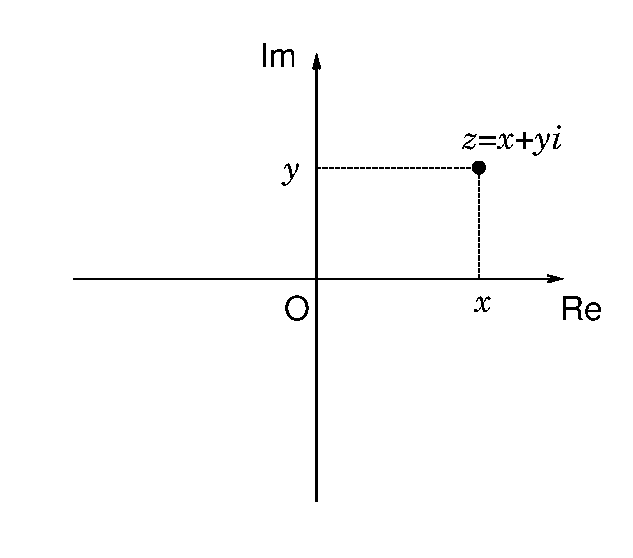
\includegraphics[width=7cm]{cplane0.eps}
    \caption{複素平面}\label{fig:cplane0}
\end{figure}

複素平面の横軸を\underline{実軸}または\underline{実数軸}と呼び, Reと表記する。
縦軸を\underline{虚軸}または\underline{虚数軸}と呼び, Imと表記する。

\begin{q}\label{q:univ_comp_plane0} $z=1+2i$のとき以下を複素平面に図示せよ。
\begin{edaenumerate}<4>
\item $z$
\item $-z$
\item $1+z$
\item $z-i$
\item $iz$
\item $z^2$
\item $1/z$
\end{edaenumerate}\end{q}

%\begin{q}\label{q:univ_comp_plane2} 
%複素平面上で, 複素数$z$とその複素共役$\overline{z}$は, 実軸に
%関して互いに対称の位置にあることを示せ。
%\end{q}\mv

ところで, 実数は数直線の上の点として, 連続的に1列に1方向に並べることが
でき, 「右に行くほど値は大きい」というふうに大小関係を定義できる。
ところが複素数は, 複素平面のように面的に並べられるものであり, 
実数のような大小関係は定義できない。従って, \textgt{虚数どうしの間とか, 
実数と虚数の間には, $<$や$>$で表される大小関係は存在しない}。
例えば, $1-i$と$-1+i$はどちらが大きいか? という問は無意味である。

\begin{faq}\label{faq:complex_plane}{\small\textgt{複素平面って, 実部と虚部を
プロットしただけですよね? 何が嬉しいのですか?}
... 本書のレベルを超える, 解析関数, 留数定理, 解析接続などという, 
大学数学を理解すれば, 複素平面の「凄さ」がわかります。興味ある人は
検索してごらん!}\end{faq}
\hv
%\begin{faq}\label{faq:complex_order}{\small\textgt{存在
%しないなら, 適当に定義を作ってしまえばいいんじゃないですか?}
%... もし実数と虚数の大小関係を定義するなら, それは実数どうしの大小関係を自然に
%含む形で拡張されなければなりません。その際, \eref{eq:axiom_order0}$\sim$
%\eref{eq:axiom_order3}という公理を満たす必要があります。そのような概念を
%うまく作ることはできないのです。}\end{faq}
%\vv



\section{複素数の絶対値}
複素数
\begin{eqnarray}z=x+iy\label{eq:complex_x_iy}\end{eqnarray}
について($x, y$は実数), $z$の\underline{絶対値} \index{ぜったいち@絶対値}
と呼ばれる量$|z|$を次式のように定義する:
\begin{eqnarray}|z|:=\sqrt{x^2+y^2}\label{eq:def_abs_complex}\end{eqnarray}

\begin{exmpl} $|1+2i|=\sqrt{1^2+2^2}=\sqrt{5}$ (例おわり)\end{exmpl}
\mv

\begin{freqmiss}{\small\textgt{上の例で, $1+2i=\sqrt{5}$と書いてしまう} ...
絶対値記号「$|$ $|$」を忘れてるよ!}\end{freqmiss}
\mv

\eref{eq:complex_x_iy}で, $y=0$, つまり$z$が実数$x$である場合, 
\eref{eq:def_abs_complex}より, 
\begin{eqnarray}|z|=\sqrt{x^2}\end{eqnarray}
となる。これは実数の意味での絶対値$|x|$と等しい。つまり複素数の絶対値は, 
実数の絶対値を自然に拡張している。だから, 実数の絶対値記号と
複素数の絶対値記号が同じ$|\quad|$でかぶっていることに, 何の問題もない。

\begin{exmpl} $-4$をあえて複素数とみなして, その絶対値を求めてみよう:
\begin{eqnarray*}|-4|=|-4+0i|=\sqrt{(-4)^2+0^2}=\sqrt{16}=4\end{eqnarray*}
これは$-4$の, 実数としての絶対値と同じ。(例おわり)
\end{exmpl}

「ピタゴラスの定理」を使えば, $|z|$は複素平面において原点から$z$までの距離である。
この観点でも, \ref{sec:realnum_calc}節で学んだ, 「実数の絶対値は原点から
その実数までの距離」という考え方の自然な拡張になっている。

\begin{comment}

\begin{q}\label{q:univ_comp_plane4} $z$を複素数とし, その複素共役を$\overline{z}$とする。以下を示せ:
\begin{edaenumerate}
\item $|\overline{z}|=|z|$
\item $z\overline{z}=|z|^2$
\end{edaenumerate}\end{q}
\mv

さて, 任意の2つの複素数$z, w$について次式が成り立つ:
\begin{eqnarray}|zw|=|z|\,|w|\label{eq:abs_zw_absz_absw}\end{eqnarray}
証明: $z=a+bi, w=c+di$とする ($a, b, c, d$は実数)。
\begin{eqnarray}
|zw|&=&|(a+bi)(c+di)|=|ac-bd+(ad+bc)i|\nonumber\\
&=&\sqrt{(ac-bd)^2+(ad+bc)^2}\nonumber\\
&=&\sqrt{a^2c^2-2abcd+b^2d^2+a^2d^2+2abcd+b^2c^2}\nonumber\\
&=&\sqrt{a^2c^2+b^2d^2+a^2d^2+b^2c^2}\label{eq:abs_zw_absz_absw1}
\end{eqnarray}
一方, 
\begin{eqnarray*}
|z|\,|w|&=&|a+bi|\,|c+di|\nonumber\\
&=&\sqrt{a^2+b^2}\sqrt{c^2+d^2}=\sqrt{(a^2+b^2)(c^2+d^2)}\nonumber\\
&=&\sqrt{a^2c^2+b^2d^2+a^2d^2+b^2c^2}\label{eq:abs_zw_absz_absw2}
\end{eqnarray*}
この式と\eref{eq:abs_zw_absz_absw1}より, 
\eref{eq:abs_zw_absz_absw}が成り立つ。\qed

\eref{eq:abs_zw_absz_absw}はとても便利な式である。
\mv

\begin{q}\label{q:univ_comp_abs0} 以下の複素数の絶対値を求めよ。ただし, $n$を正の整数とする。
ヒント: (3), (4)には\eref{eq:abs_zw_absz_absw}を使う。
\begin{enumerate}
\item $1+3i$
\item $i$
\item $(1+i)(1+2i)(1+3i)$
\item $(1+i)^n$
\end{enumerate}\end{q}
\mv
\begin{comment}
\begin{q}\label{q:univ_comp_abs001} 0でない任意の複素数$z$について, 次式
を証明せよ:
\begin{eqnarray}
\Bigl|\frac{1}{z}\Bigr|=\frac{1}{|z|}\label{eq:abs_frac}
\end{eqnarray}
\end{q}

\begin{q}\label{q:univ_comp_abs001} 任意の複素数$z$, $w$について, 次式
を証明せよ。ただし$w\neq0$とする。
\begin{eqnarray}
\Bigl|\frac{z}{w}\Bigr|=\frac{|z|}{|w|}\label{eq:abs_frac2}
\end{eqnarray}
\end{q}

\eref{eq:abs_frac}や\eref{eq:abs_frac2}は, 複素数の分数の
絶対値を求める時にとても便利である。これを忘れて, わざわざ有理化しようと
して苦労する, 可哀想な学生が毎年いるのだ!

\begin{q}\label{q:univ_comp_abs1} 以下の複素数の絶対値を求めよ。
ただし, $n$を正の整数とする。
\begin{edaenumerate}<3>
\item \begin{eqnarray*}\frac{1}{4+3i}\end{eqnarray*}
\item \begin{eqnarray*}\frac{1+2i}{1-2i}\end{eqnarray*}
\item \begin{eqnarray*}\frac{1}{(1-i)^n}\end{eqnarray*}
\end{edaenumerate}\end{q}

\begin{faq}{\small\textgt{複素数の絶対値って, 何の役に立つのですか?}
... 実用的には, 例えば, 電気工学や機械工学で, 電気信号の大きさや
機械の揺れの大きさを検討する時に使います。それだけじゃないけどね。

\small\textgt{でも電気や機械って, 資源には関係なくないですか?}
... 農業には農業機械や農業施設やセンサーを使うし, 食品作るのも
たくさん機械が必要です。しかも特殊なやつがね。化学や微生物の実験
でも電気や機械は必要。}\end{faq}
\hv
\end{comment}
\hv



\section{極形式}
さて, 複素平面上の点
\begin{eqnarray}z=x+iy\,\,\,\,\,\,(x, y\text{は実数})\label{eq:def_comp_z_0}\end{eqnarray}
について, $r$を原点からその点までの距離, すなわち
\begin{eqnarray}r=|z|=\sqrt{x^2+y^2}\label{eq:compnum_r}\end{eqnarray}
とし($0\le r$), $\theta$を実軸からその点までの角度($0\le\theta<2\pi$)として, 
極座標の考え方(\eref{eq:2Dpolar})を使えば, 
\begin{equation}\begin{cases}
x = \text{Re}(z)=r \cos \theta\\
y = \text{Im}(z)=r \sin \theta
\end{cases}\label{eq:compnum_x_y_r_theta}\end{equation}
と表すことができる。これを\eref{eq:def_comp_z_0}に代入すれば, 
\begin{eqnarray}
z&=&r\cos\theta+ir\sin\theta\nonumber\\
 &=&r(\cos\theta+i\sin\theta)
\end{eqnarray}
となる。ここで()の中はオイラーの公式
(\eref{eq:EulerFormula})より$e^{i\theta}$と書くことができるので, 結局, 
\begin{eqnarray}
z=re^{i\theta}\label{eq:comppolar}
\end{eqnarray}
と表すことができる。このように, 任意の複素数は, 0以上の実数$r$と0から$2\pi$までの実数$\theta$の組合せで表現する
ことができる。この表現形式を\underline{極形式} \index{きょくけいしき@極形式}と呼ぶ。対照的に, 
これまで馴染み深かった, $z=x+iy$のように表す表現形式を, \underline{座標形式}と呼ぶ。
同じ複素数を, 座標形式と極形式という2通りの形式で表現できるのだ。\mv

複素数の極形式$re^{i\theta}$について, $r$を\underline{動径} \index{どうけい@動径}, $\theta$を
\underline{偏角} \index{へんかく@偏角}とか\underline{位相} \index{いそう@位相}と呼ぶこともある。

\begin{exmpl} 複素数$z=3+\sqrt{3}\,i$を, 極形式で表してみよう。この複素数を複素平面に
プロットすると, 図\ref{fig:cplane_exm}のようになる。
\begin{figure}[h]
    \centering
    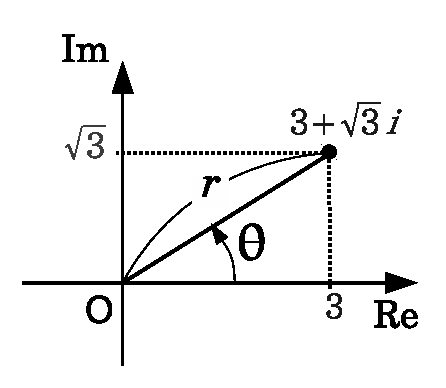
\includegraphics[width=4cm]{cplane_exm.eps}
    \caption{$z=3+\sqrt{3}i$を複素平面にプロット。}\label{fig:cplane_exm}
\end{figure}
この場合, \eref{eq:compnum_r}より, 動径は, 
\begin{eqnarray}r=|z|=\sqrt{3^2+(\sqrt{3})^2}=\sqrt{12}=2\sqrt{3}\end{eqnarray}
となる。また, \eref{eq:compnum_x_y_r_theta}より, 
\begin{eqnarray*}
&&\text{Re}(z)=3=r \cos \theta = 2\sqrt{3}\cos\theta\\
&&\text{Im}(z)=\sqrt{3}=r \sin \theta = 2\sqrt{3}\sin \theta
\end{eqnarray*}
なので, 
\begin{eqnarray}
\cos\theta=\frac{3}{2\sqrt{3}}=\frac{\sqrt{3}}{2},\quad
\sin\theta=\frac{\sqrt{3}}{2\sqrt{3}}=\frac{1}{2}
\end{eqnarray}
となる。これを満たすのは$\theta=\pi/6$である。従って, 
\begin{eqnarray}
z=2\sqrt{3}\,e^{i\pi/6}
\end{eqnarray}
となる。(例おわり)
\end{exmpl}
\hv

極形式から座標形式に変換するには, \eref{eq:compnum_x_y_r_theta}を使って$x$と$y$を求め, \eref{eq:def_comp_z_0}でまとめればよい。\\

\begin{q}\label{q:univ_comp_polar0} 以下の複素数について, 極形式は座標形式に, 座標形式は極形式に変換せよ。
\begin{edaenumerate}<3>
\item $z=1+i$
\item $z=\sqrt{3}+i$
\item $z=-i$
\item $z=e^{i\pi/4}$
\item $z=2e^{i\pi}$
\item $z=2 e^{i\pi/3}$
\end{edaenumerate}\end{q}
\vspace{0.3cm}

\begin{q}\label{q:univ_comp_polar2} 以下の計算を行い, 結果を極形式で示せ。(指数法則を使ってよい)
\begin{edaenumerate}
\item $e^{i\pi/4}\times e^{i\pi/3}$
\item $e^{i\pi/4}/e^{i\pi/3}$
\item $e^{i\pi/4}\times i$
\item $(e^{i\pi/4})^2$
\item $(2e^{i\pi/3})^3$
\end{edaenumerate}\end{q}
\vspace{0.3cm}

\begin{q}\label{q:univ_comp_polar_abs} 極形式を用いて次式を
証明せよ。
\begin{eqnarray}|zw|=|z|\,|w|\label{eq:abs_zw_absz_absw}\end{eqnarray}
\end{q}
\vspace{0.3cm}

このように, 極形式を使うと, 座標形式に較べて, 複素数の掛け算・割り算が非常にシンプルになる。
すなわち, 2つの複素数の掛け算は動径どうしの掛け算と偏角どうしの足し算だし, 
2つの複素数の割り算は動径どうしの割り算と偏角どうしの
引き算である。そして, 偏角の足し算や引き算は, 原点を中心とする回転に相当する。

一方, 複素数の足し算・引き算については, 極形式は不便であり, 座標形式のほうが簡単になる。問題の
状況にあわせて, 座標形式と極形式のどちらを使うか, 適切に判断することが重要である。それができれば, 
複素数の扱いはとても楽になる。\\

\begin{q}\label{q:univ_comp_polar4} 複素数$z$, 実数$r$, $\theta$, $\alpha$について,
\begin{enumerate}
\item $z$に$e^{i\alpha}$を掛けると, 複素平面上の$z$の位置が, 原点を中心に$\alpha$だけ左向きに回転することを示せ。
\item $z=re^{i\theta}$とすると, $\overline{z}=re^{-i\theta}$であることを示せ。
\end{enumerate}\end{q}
\mv

\begin{exmpl} $e$以外の数の虚数乗を考えてみよう。例えば$4^i$は何だろうか? $4=e^{\ln 4}$なので, 
\begin{eqnarray*}
4^i&=&(e^{\ln 4})^i=e^{(\ln 4)i}=\cos(\ln 4)+i\sin(\ln 4)\\
   &\fallingdotseq&\cos(1.386)+i\sin(1.386)\fallingdotseq0.1835+0.9830i
\end{eqnarray*}
(例おわり)\end{exmpl}
\hv

\begin{q}\label{q:univ_comp_i_pow_i} $i^i$を求めてみよう:
\begin{enumerate}
\item $i=e^{\pi i/2}$であることを示せ。
\item $i^i=e^{-\pi/2}$であることを示せ。
\item (2)の結果と電卓を使って, $i^i\fallingdotseq 0.2079$であることを示せ。
\end{enumerate}\end{q}
\mv


\begin{comment}

ここで, 複素数の操作について, まとめておこう。
\vspace{0.3cm}

複素数の演算と, それに対応する複素平面上での操作
\begin{itemize}
\item 足し算・引き算:ベクトルの足し算・引き算と同じ。計算は座標形式が楽。
\item 掛け算:動径の掛け算と偏角の足し算。計算は極形式が楽。
\item 割り算:動径の割り算と偏角の引き算。計算は極形式が楽。
\item $e^{i\theta}$を掛ける:$\theta$だけ, 左に回転
\item $e^{-i\theta}$を掛ける:$\theta$だけ, 右に回転
\item $i$を掛ける:90度, 左に回転
\item $-1$を掛ける:原点に関して対称移動(180度回転)
\item 複素共役:実軸に関して対称移動(上下反転)
\end{itemize}
\vspace{0.3cm}

複素共役の求め方
\begin{itemize}
\item 複素共役=座標形式で, 虚部の符号を逆に  ($x-yi$)
\item 複素共役=極形式で, 動径はそのままで偏角の符号を逆に ($re^{-i\theta}$)
\item 積の共役は共役の積。\eref{eq:compconj_z_times_w} ($\overline{z_1 z_2}=\overline{z_1}\cdot\overline{z_2}$)
\end{itemize}
\vspace{0.3cm}

複素数の絶対値の求め方
\begin{itemize}
\item 絶対値=(実部)$^2+$(虚部)$^2$の平方根  ($\sqrt{x^2+y^2}$)
\item 絶対値=動径 ($re^{i\theta}$の$r$)
\item 絶対値=複素共役との積の平方根  ($\sqrt{z\overline{z}}$)
\item 積の絶対値は絶対値の積。 ($|z_1 z_2|=|z_1|\cdot|z_2|$)
\item 分数の絶対値は, 分子の絶対値/分母の絶対値。  ($|z_1/z_2|=|z_1|/|z_2|$)
\item $e^{i\theta}$の絶対値は, $\theta$によらず1。 ($|e^{i\theta}|=1$)
\end{itemize}
\vspace{0.3cm}

\begin{q}\label{q:univ_comp_polar6} 以下の複素数の絶対値を求めよ
\begin{edaenumerate}
\item $e^{i\pi/3}$
\item $e^{i\pi/3}-e^{-i\pi/3}$
\item $(e^{\pi i/4})^3$
\item $e^{i\pi/5}\times e^{i2\pi/7}\times e^{i3\pi/11}$
\item $e^{i\pi/6}+e^{-i\pi/6}$
\item $(2e^{i\pi/6})^3$
\end{edaenumerate}\end{q}

\begin{freqmiss}{\small\textgt{絶対値記号「$||$」を省略し, 複素数とその絶対値を
イコールで結んでしまう。例えば, 問\ref{q:univ_comp_polar6}(4)で, 
$e^{i\pi/5}\times e^{i2\pi/7}\times e^{i3\pi/11}=1$と書いてしまう。}}\end{freqmiss}
\vv
\end{comment}




\section{偏微分}
多変数関数において, ある特定の変数についてのみ微分することを, \underline{偏微分}
(partial derivative)とか\underline{偏導関数}と呼ぶ。
\index{へんびぶん@偏微分}\index{へんどうかんすう@偏導関数}そのとき, 他の変数は定数とみなされる。

\begin{exmpl}$f(x,y)=xy^2+3x$を, $x$について偏微分すると, $y$を定数とみなして, 
\begin{eqnarray*} \frac{\partial f}{\partial x} = y^2+3 \end{eqnarray*}
となる。$y$について偏微分すると, $x$を定数とみなして, 
\begin{eqnarray*} \frac{\partial f}{\partial y} = 2xy \end{eqnarray*}
となる。(例おわり)\end{exmpl}

$\partial$は偏微分を表現するための記号であり, 「ラウンドディー」とか「ラウンド」
などと呼ばれる。書く時は, 数字の$6$を左右逆にすればOK。
\begin{freqmiss}{\small\textgt{偏微分記号$\partial$を正しく書けない。
間違いでよくあるのが, $\delta$とか$\sigma$とか6。}}\end{freqmiss}

\begin{q}\label{q:univ_part_deriv0} 以下の関数を$x, y$のそれぞれで偏微分せよ:
\begin{edaenumerate}
\item $f(x,y)=x^2+y^2$
\item $f(x,y)=\exp(xy)$
\item \begin{eqnarray*}f(x,y)=\sqrt{x^2+y^2}\,\,\,\,\,\,\end{eqnarray*}
\item \begin{eqnarray*}f(x,y)=\frac{1}{\sqrt{x^2+y^2}}\,\,\,\,\,\,\end{eqnarray*}
\end{edaenumerate}\end{q}
\mv

偏微分を, 何回も繰り返すことがある。それを高階の偏微分という。高階の偏微分は, 複数の変数
について行うことがある。\\

\begin{exmpl} $\,\,\,\,f(x,y)=\exp(xy)$について, 
\begin{eqnarray}
&&\frac{\partial f}{\partial x}=y\exp(xy)\\
&&\frac{\partial^2 f}{\partial x^2}=y^2\exp(xy)\\
&&\frac{\partial^2 f}{\partial y \partial x}=\frac{\partial}{\partial y}\frac{\partial f}{\partial x}=xy\exp(xy)+\exp(xy)
\end{eqnarray}
(例おわり)\end{exmpl}
\mv

ところで, 興味深いことに, 多くの関数について, 
\begin{equation}
\frac{\partial^2 f}{\partial y \partial x}=\frac{\partial^2 f}{\partial x \partial y}
\label{eq:pderivorder}
\end{equation}
が成り立つ。\\

\begin{q}\label{q:univ_part_deriv2} $f(x,y)=\exp(xy)$について, 
\eref{eq:pderivorder}が成り立つことを確認せよ。
\end{q}\mv

\begin{q}\label{q:univ_part_deriv4} $f(x,y)=(e^y+e^{-y}) \cos x$について, 
\begin{enumerate}
\item $\partial^2 f/\partial x^2$を求めよ。
\item $\partial^2 f/\partial y^2$を求めよ。
\item 以下の式が成り立つことを示せ\footnote{\eref{eq:2DLaplace}は, 2次元ラプラス方程式という偏微分方程式
である。応用上, 重要な方程式である。}:
\begin{eqnarray}
\frac{\partial^2 f}{\partial x^2}+\frac{\partial^2 f}{\partial y^2}=0
\label{eq:2DLaplace}\end{eqnarray}
\end{enumerate}\end{q}
\vv

\begin{faq}{\small\textgt{\eref{eq:pderivorder}が
「多くの関数について成り立つ」とありますが, 成り立たないのはどんな関数ですか?}\\
... 例えば, $f(x, y)=x+|y|$は, 
\begin{eqnarray*}
\frac{\partial f}{\partial x}=1,\,\,\,\,\,
\frac{\partial^2 f}{\partial y\partial x}=0
\end{eqnarray*}
となりますが, $y=0$では$\partial f/\partial y$が存在しないので, 
$\partial^2 f/\partial x\partial y$も存在しません。従って, 
\eref{eq:pderivorder}は$y=0$で成り立ちません。}\end{faq}
\vv


\section{全微分}

1変数関数の微分は, \peref{eq:define_dif}で定義される。これを多変数関数に拡張しよう。

2つの変数$x, y$の関数$f(x,y)$について, $(x, y)$と, それに非常に近い点$(x+dx, y+dy)$の
間で, $f$はどのような関係にあるだろうか? 

まず, $f(x,y)$を$x$だけの関数だとみなし, $\partial f/\partial x$を$f_x$とかけば, 微分の定義から, 
\begin{eqnarray*}f(x+dx,y+dy) = f(x,y+dy) + f_x(x, y+dy)dx\end{eqnarray*}
となる。また, この右辺の$f(x,y+dy)$を$y$だけの関数とみなし, $\partial f/\partial y$を$f_y$とかけば, 
$y$による微分の定義から, 
\begin{eqnarray*}f(x,y+dy) = f(x, y) + f_y(x, y)dy\end{eqnarray*}
従って, 
\begin{eqnarray*}
&&f(x+dx,y+dy)\\
&&= f(x, y) + f_x(x, y+dy)dx + f_y(x, y)dy\end{eqnarray*}
となる。この右辺第2項について, $y+dy$は$y$とほとんど同じと考えれば, 
\begin{eqnarray*}f_x(x, y+dy)dx = f_x(x, y)dx\end{eqnarray*}
となり, 従って, 
\begin{eqnarray*}f(x+dx,y+dy) = f(x, y) + f_x(x, y)dx + f_y(x, y)dy\end{eqnarray*}
となる。すなわち, 
%\begin{itembox}{2変数の全微分公式}
\begin{eqnarray}
f(x+dx,y+dy) = f(x, y)+ \frac{\partial f}{\partial x}dx+\frac{\partial f}{\partial y}dy\nonumber\\
\label{eq:def_2var_zenbibun}\end{eqnarray}
%\end{itembox}
と書ける。これを\underline{全微分公式}もしくは簡単に\underline{全微分}\index{ぜんびぶん@全微分}と呼ぶ。
この式は, 1変数関数の微分係数の定義式, すなわち\peref{eq:define_dif}を, 形式的に素直に
2変数関数に拡張した形になっていることがわかるだろう。

ここで, 
\begin{eqnarray}df=f(x+dx,y+dy) - f(x, y)\end{eqnarray}
とすれば, \eref{eq:def_2var_zenbibun}は
\begin{eqnarray}
df= \frac{\partial f}{\partial x}dx+\frac{\partial f}{\partial y}dy
\end{eqnarray}
となる。この式は\peref{eq:define_dif001}を2変数関数に拡張した形をしている。\\

全微分公式は, もっとたくさん変数を持つ関数にも拡張される。すなわち, $f(x, y, z, \cdots)$に対して, 
\begin{eqnarray*}df=f(x+dx, y+dy, z+dz, \cdots) - f(x, y, z, \cdots)\end{eqnarray*}
とすれば, 
\begin{eqnarray}
df = \frac{\partial f}{\partial x}\,dx + \frac{\partial f}{\partial y}\,dy + \frac{\partial f}{\partial z}\,dz\ + \cdots
\end{eqnarray}
となる。こうなる理由は, 上の2変数の場合から類推できるだろう。

全微分は, 多変数関数を$dx$や$dy$の一次式で近似すること, すなわち
「線型近似」の多変数バージョンである。全微分はとても実用的な公式だ。
ある関数の変化や誤差が, 各変数の変化や誤差にどのように依存するかを, 教えてくれるのだ。\\

\begin{faq}{\small\textgt{$\partial$は偏微分の記号ですが, ならば
全微分を表す記号は無いのですか?} ... 全微分は言葉(というか式)だけで, 
「全微分を表す記号」はありません。}\end{faq}\mv


\begin{q}\label{q:univ_deriv_gas} 理想気体の状態方程式:$P=\rho RT$を考える。$\rho$はモル密度(単位体積あたりのモル数), 
$R$は気体定数(8.31 J mol$^{-1}$ K$^{-1}$)である。摂氏0度(273 K), 1000 hPa ($1 \times 10^{5}$ Pa)の
状態から, 温度を摂氏1度, 圧力を1001 hPaにすると, この気体のモル密度はどのくらい変わるか調べよう。
\begin {enumerate}
\item 最初の状態での$\rho$を, そのときの$T, P$から計算せよ(電卓!)。
\item 次の状態での$\rho$を, そのときの$T, P$から計算せよ(電卓!)。
\item それらの差を求めよ。
\item これを全微分でやってみよう。まず次式を示せ:
\begin{eqnarray}d\rho=\frac{1}{RT}dP-\frac{P}{RT^2}dT\end{eqnarray}
\item $T, P$は最初の状態とし,
\begin{eqnarray}dT=1\,\text{K},\,\,\,\, dP=1\,\text{hPa}=10^2\,\text{Pa}\end{eqnarray}
として, 上の式を計算して$d\rho$を求めよ。
\end{enumerate}\end{q}

\begin{faq}{\small\textgt{1変数の微分では直線の式が出てきて,2変数の全微分では
平面の式が出てくるということ?} 
... そうです。2変数関数$z=F(x, y)$を全微分すると,
\begin{eqnarray*}
z=F(x+dx, y+dy)=F(x, y)+\frac{\partial F}{\partial x}dx+\frac{\partial F}{\partial y}dy
\end{eqnarray*}
となりますが, ここで$dx, dy, z$を変数, 残りを定数とみなせば, これは
平面を表す方程式です(あとで「ベクトル」の章でやります)。}\end{faq}
\mv


\begin{faq}{\small\textgt{全微分と偏微分は微生物系に進む人にも必要ですか?}
... 微生物研究でも必要な場合が多くありますし, 理解していた方が結果の考察がやり
やすい場面が多いです。具体的に言うと, 微生物を使用して何かの物質を大量に作る
(プラント)場合(発酵学や醸造学)など環境条件と微生物の増殖速度, 得られる物質
の収量などを解析する際(一種のモデリングです)に, 必要になります。またこれと
同様の解析方法を要求されるのが, 微生物を利用した廃水処理プラントです。さらに, 
湖や湖沼での物質収支モデル構築にも必要です。こういった研究を将来やりたいと
考えているのであれば, 全微分や偏微分の知識があると必ず役立ちます。
また, 近年盛んになってきている蛍光色素を利用した細胞検出や遺伝子検出など
の際にも全微分や偏微分の知識があると役立ちます。
微生物研究でも生態的な研究を行いたい場合には, 環境に関する研究ですので, 
広範な知識と解析方法を持っていることが非常に有利に働きます。例えば, 
海洋での微生物研究を行う際には, 海洋物理に相当する表層だけでない海流など
の動きのシミュレートと栄養塩類濃度分布, 微生物量などの関係を解析しますが, 
上記海洋物理の知識もある程度必要ですので, やはり全微分や偏微分の知識が
あると役立つと思います。
実際に, 私が昨年乗船した北極海調査では, 数名の海洋物理学の研究者も乗船
しており, 船上に上がってくるリアルタイムのデータをすぐに解析して, 海中環境
(物理的&化学的)の議論をすること多々でした。(内海真生先生)}\end{faq}
\mv


\section{面積分と体積分}\label{sect:mensekibun}

ここで, ちょっと変わった積分を学ぼう。それは, 微小量が面積や体積になる
ような積分である。どういうものなのか, 以下の例を見て欲しい:

\begin{exmpl}君は広くて平坦で長方形の農場を持っている。
図\ref{fig:farm}のように地面に$xy$座標系を設定し, 
\begin{eqnarray*}
0\le x\le X\\
0\le y\le Y
\end{eqnarray*}
の範囲がこの農場であるとしよう。農場の
面積$S$は, もちろん$S=XY$となる。

さて, この農場に雨が降る。広いので, 雨の強さは均一でなく場所ごとに違う。
すると, 君の農場全体に, 単位時間あたりに降る雨量(つまり雨水の体積/時間)$R$
をどうやって見積もればよいだろう? 図\ref{fig:farm}のように
農場を$x$方向に$n$列, $y$方向に$m$列が
できるような格子状に分割すると, 合計$mn$個の小さな長方形の農地ができる。
$x$方向に$i$番め, $y$方向に$j$番めにある小農地に降る単位時間あたりの雨量
を$\Delta R(x_i, y_j)$としよう。すると, 全農場に降る単位時間あたりの雨量$R$は, 
各小農地に降る単位時間あたりの雨量の合計だから, 
\begin{eqnarray}
R=\sum_{j=1}^{m}\sum_{i=1}^{n}\Delta R(x_i, y_j)\label{eq:farm0}
\end{eqnarray}
となる(当たり前である)。

\begin{figure}[h]
    \centering
    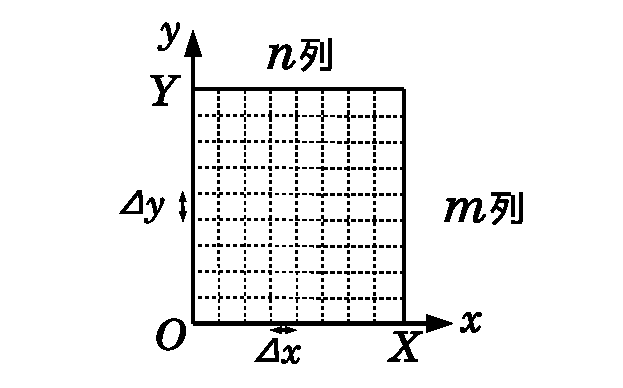
\includegraphics[width=9cm]{farm.eps}
    \caption{君の農場}
\label{fig:farm}
\end{figure}

さて, 分割の数, つまり$m$や$n$をたくさんとれば, 各小農地はいくらでも小さくできる。
すると, それぞれの小農地の中では, 雨の強さがほとんど均一とみなせる
だろう。点$(x, y)$の付近で, 単位面積あたりに降る雨量を$F(x, y)$
とすると, $F(x, y)$は2つの独立変数$(x, y)$に関する関数である。すると, 
\begin{eqnarray}
\Delta R(x_i, y_j)\fallingdotseq F(x_i, y_j)\Delta S_{ij}\label{eq:farm1}
\end{eqnarray}
となる。ここで$\Delta S_{ij}$は, この小農地の面積とする。すると式(\ref{eq:farm0})は,
\begin{eqnarray}
R\fallingdotseq \sum_{j=1}^{m}\sum_{i=1}^{n}F(x_i, y_j)\Delta S_{ij}\label{eq:farm15}
\end{eqnarray}
となる。ここで分割を限りなく細かくすると, $n$と$m$は$\infty$に行き, $\sum$は$\int$
に変わり, $\Delta S_{ij}$は$dS$に変わり, $\fallingdotseq$は$=$に変わる:
\begin{eqnarray}
R = \int\int_{\text{農場}}F(x, y)\,dS\label{eq:farm2}
\end{eqnarray}
ここで積分記号の下に「農場」と書いたのは, 農場全体で分割と和を行う, という
意味である(積分区間を書く代わり)。

これでもいいのだが, \eref{eq:farm1}に戻ってもう少し考えてみよう。
小農地の$x$方向の長さを$\Delta x$, $y$方向の長さを$\Delta y$とすると, もちろん
\begin{eqnarray}
\Delta S_{ij}=\Delta x\,\Delta y\label{eq:farm25}
\end{eqnarray}
である\footnote{むろん, $\Delta x=X/n$, $\Delta y=Y/m$である}。すると, \eref{eq:farm15}は, 
\begin{eqnarray}
R\fallingdotseq \sum_{j=1}^{m}\sum_{i=1}^{n}F(x_i, y_j)\Delta x\Delta y\label{eq:farm3}
\end{eqnarray}
となり, $\Delta x$と$\Delta y$を0に, $n$と$m$を無限大に持っていけば, 
\begin{eqnarray}
R=\int_{0}^{Y}\int_{0}^{X}F(x, y)\,dx\,dy\,\label{eq:farm7}
\end{eqnarray}
になる。(例おわり)\end{exmpl}

\eref{eq:farm2}や\eref{eq:farm7}のように, 積分記号が2つ以上出てくるような積分のことを
重積分\index{じゅうせきぶん@重積分}とか多重積分\index{たじゅうせきぶん@多重積分}とよぶ。
特に, この例のように, 平面図形を無数の小さな図形に分割し, それぞれの微小面積を関数にかけて
足し合わせる場合は2重積分になり, そのことを特に面積分\index{めんせきぶん@面積分}と呼ぶ。
同様に, 立体を無数の小さな立体に分割し, それぞれの微小体積を関数にかけて
足し合わせる場合は3重積分になり, そのことを特に体積分\index{たいせきぶん@体積分}と呼ぶ。\\

面積分や体積分は, 積分範囲(上の例では, 畑の形)が単純な長方形や直方体であり, 
なおかつ被積分関数が$x$と$y$(と$z$)の簡単な関数で表される場合は, それぞれの
変数で順番に計算していけばよい(そうでない場合は難しくなる)。

\begin{q}\label{q:mensekibun01} 以下の面積分を計算せよ。
ヒント: まず被積分関数を$x$だけの関数とみなして($y$は定数とみなして)
$x$で定積分し(その結果は$x$を含まない$y$だけの式になる), 次に$y$で定積分する。
\begin{eqnarray}
\int_{-2}^{2}\int_{0}^{3}(x^2+xy)dxdy
\end{eqnarray}
\end{q}
\mv

\begin{faq}{\small\textgt{重積分って難しそうです。ただの積分も難しい
のに, それがダブルで来たりしたらもう...} ... そんなに難しく考えなくて
OK! ふつうの積分は, 関数に, 線(数直線)を分割した微小量をかけて足す
ことで, 面積分は, 面(平面図形)を分割した微小量をかけて足すことです。
概念的には大差ない。}\end{faq}
\mv

\begin{faq}{\small\textgt{でも, 重積分の計算ってどうやるのですか?}
 ... 面積分や体積分を実際に「計算せよ」ということは少なく, 
むしろ面積分や体積分は, 現象を語る表現手段として現れることの
方が多いです。その例が\eref{eq:farm7}。この式は, 「畑に降った雨の総量」
を表現しているけど, 実際にその値をここでは求めてはいません。もちろん, 
具体的な$F(x, y)$がわかるなら, その積分を実行すれば雨量は求まります
が, それには普通, コンピュータを使います。しかし\eref{eq:farm7}
は, それ自体が「ある概念を表す」という点で, 十分に意味ある式なのです。}\end{faq}
\mv

\begin{faq}{\small\textgt{大学の数学は哲学みたいだと聞いていましたが
その通りだと思いました。} ... そのあたりの気持ちの切り替えは必要ですね。
問題が解けること以上に, 論理と概念を理解することの方が重要になってきます。}\end{faq}
\mv

\begin{q}\label{q:integ_okashi0} ある直方体状のお菓子の
砂糖の濃度は, 部位によって異なる。場所$(x, y, z)$における
砂糖の濃度(単位体積あたりに含まれる砂糖の質量)を
$C(x, y, z)$とする。このお菓子全体に含まれる砂糖の量$S$
を表す式を述べよ。直方体は, $0\leq x\leq a$, $0\leq y\leq b$, $0\leq z\leq c$
の領域とする。
\end{q}
\hv



\section{関数と無次元量}\label{sect:func_and_dimless}

既に学んだように, 
$\sin x$は, 以下のように無限次の多項式でマクローリン展開できる:
\begin{eqnarray}
&&\sin x = \frac{x}{1!}-\frac{x^3}{3!}+\frac{x^5}{5!}-\frac{x^7}{7!}+\cdots\label{eq:Taylor_sin8}
\end{eqnarray}
ここで, もし$x$に何らかの次元があれば, 困ったことになる。実際, 
$x$がもし「長さ」という次元を持ち, mという単位で表されるなら, 
$x^3$はm$^3$という単位を持つ。ところが, mという単位を持つ量とm$^3$
という単位を持つ量を足すことはできない(異なる次元の量は足せない)。
従って, \eref{eq:Taylor_sin8}の右辺が意味を持つのは, 
$x$が無次元量(単位を持たない量)であるときに限る。
従って, 現実的には, $\sin x$のような関数の引数(関数に入れる数, つまり独立変数)
は, 無次元量でなければ意味がないのである。そこで, 現実的な問題を扱う科学では, 
このような関数の引数を無次元にするために, 何らかの定数を掛けたり割ったりして, 
つじつまをあわせる必要がある。

\begin{exmpl}
\pref{eq:trig_harmonic_oscilation}では, 単振動の式:
\begin{eqnarray}
x(t)=x_0\cos(\omega t + \delta)\label{eq:trig_harmonic_oscilation_again}
\end{eqnarray}
を学んだ($t$は時刻, $\omega$は角速度, $\delta$は適当な定数)。既に学んだように, 
$\cos\theta$も$\theta$に関する無限次の多項式でマクローリン展開されるので, 
引数$\theta$は無次元量でなくてはならない。ところが$t$は「時間」という
次元を持ち, 「秒」などの単位で表される。そこで, それを無次元にする(単位を消す)
ために, $\omega$という係数が必要なのだ。このことから, $\omega$が
「1/時間」の次元を持ち, s$^{-1}$などの単位で表されるということがすぐわかる。
同様に$\delta$も無次元量である(「初期位相」と呼ばれる)。(例おわり)\end{exmpl}

もちろん, $\omega$は角速度という, 立派な意味を持つ量であり, 
単なるつじつまあわせの為だけに存在するのではない。しかし, 数学的な形式と, 
量の次元(単位)の整合性だけに着目しても, このようにいろいろなことがわかるのである。
\hv


\section*{演習問題}

\begin{exq}\label{q:integ_okashi} あるお菓子は半径$R$の球形をしており, 
中の方が甘い。お菓子の中の砂糖の濃度を$C$とすると, $C$は中心で最大値
$C_{\,0}$をとり, 表面で0である。中心から表面までは, $C$は中心からの
距離$r$に関する一次関数で表されるとする。このお菓子
に含まれる砂糖の全質量を表す式を導け。それは, このお菓子と同じ形・大きさで, 砂糖が
濃度$C_{\,0}$で均一に存在するような別のお菓子に含まれる砂糖の全量の何倍に相当するか? 
ヒント: 中心から半径$r$, 厚さ$dr$の球殻に含まれる
砂糖の質量は? それを足し合わせれば(すなわち積分すれば)よい。
\end{exq}
\mv

\begin{exq}\label{q:univ_Taylor5} テーラー展開を直接せずに(\eref{eq:univ_Taylor4}などを使って), 次式を示せ:
\begin{eqnarray}
&&\frac{1}{1+x}=1-x+x^2-x^3+x^4-x^5+\cdots\label{eq:univ_Taylor51}\\
&&\ln (1+x)=x-\frac{x^2}{2}+\frac{x^3}{3}-\frac{x^4}{4}+\cdots\label{eq:univ_Taylor52}\\
&&\frac{1}{1+x^2}=1-x^2+x^4-x^6+x^8-\cdots\label{eq:univ_Taylor53}\\
&&\arctan x=x-\frac{x^3}{3}+\frac{x^5}{5}-\frac{x^7}{7}+\frac{x^9}{9}-\cdots\label{eq:univ_Taylor54}\\
&&1-\frac{1}{3}+\frac{1}{5}-\frac{1}{7}+\frac{1}{9}-\cdots=\frac{\pi}{4}\label{eq:univ_Taylor55}
\end{eqnarray}
{\small ヒント: \eref{eq:univ_Taylor51}は, \eref{eq:univ_Taylor4}をちょっと
工夫。\eref{eq:univ_Taylor52}は\eref{eq:univ_Taylor51}の両辺を不定積分して
$x=0$でつじつまが合うようにすれば出てくる。\eref{eq:univ_Taylor51}
の$x$に$x^2$を代入すると\eref{eq:univ_Taylor53}。\eref{eq:univ_Taylor53}の
両辺を不定積分して$x=0$でつじつまが合うようにすれば\eref{eq:univ_Taylor54}。
\eref{eq:univ_Taylor54}の両辺に$x=1$を代入すると, \eref{eq:univ_Taylor55}
($x=1$は, もとの\eref{eq:univ_Taylor4}の収束半径のぎりぎり端っこであって, 
内側ではないが, \eref{eq:univ_Taylor54}の収束半径の内側には入っている)。}
\end{exq}
\mv

\begin{exq}\label{q:univ_Taylor7} テーラー展開を直接行なって, \eref{eq:univ_Taylor51}, 
\eref{eq:univ_Taylor52}, \eref{eq:univ_Taylor53}, \eref{eq:univ_Taylor54}
を示せ。\end{exq}
\mv


\begin{exq}\label{q:funct_dim_seigou} 以下の関数で, $x$が無次元量でなければ意味を
持たないものを選び, その理由を述べよ。 ヒント: 1は無次元量である。
\begin{edaenumerate}<3>
\item $x^2$
\item $1/x$
\item $1+x$
\item $1/(1-x)$
\item $\tan x$
\item $\exp x$
\item $\ln x$
\end{edaenumerate}\end{exq}
\hv










\section*{問題の解答}

% 解答: テーラー展開

\noindent{\textbf{答}}\ref{eq:Maclaurin_linear_approx} \eref{eq:macl}
で, $x^2$以降の項を無視すると, 線型近似の式に一致する。すなわち, 
\eref{eq:macl}は, 線型近似の式に, さらに高次の項を付け加えたもの
と見ることができる。\mv

% 2011.0906 ヤマサキ解答追加。以下2問。
\noindent{\textbf{答}}\ref{q:univ_Taylor0}
$f(x)=e^x$と置くと, $f(0)=e^0=1, f'(0)=e^0=1, f''(0)=e^0=1,\,\,\cdots$であるので, これらを\eref{eq:Taylor_expansion}に代入すると, 
\begin{eqnarray*}
e^x &=& \frac{1}{0!} + \frac{1}{1!}\,x\, + \frac{1}{2!}\,x^2 + \frac{1}{3!}\,x^3 + \frac{1}{4!}\,x^4 +\,\, \cdots \\
&=& \frac{1}{0!}\,+\,\frac{x}{1!}\, +\,\frac{x^2}{2!}\,+\,\frac{x^3}{3!}\,+\,\frac{x^4}{4!}\,+\,\, \cdots \\
\end{eqnarray*}

$f(x)=\sin x$と置くと, $f(0)=\sin 0 = 0, f'(0)=\cos 0 = 1, f''(0)=-\sin 0 = 0, f'''(0)=-\cos 0= -1 , f''''(0) = \sin 0 = 0 \,\,\cdots$であるので, これらを\eref{eq:Taylor_expansion}に代入すると, 
\begin{eqnarray*}
\sin x &=& \frac{0}{0!} + \frac{1}{1!}\,x\, + \frac{0}{2!}\,x^2 + \frac{(-1)}{3!}\,x^3 + \frac{0}{4!}\,x^4 + \frac{1}{5!}\,x^5\,+\,\, \cdots \\
&=& \frac{x}{1!}\,-\,\frac{x^3}{3!}\,+\,\frac{x^5}{5!}\,-\,\frac{x^7}{7!}\,\, \cdots \\
\end{eqnarray*}

$f(x)=\cos x$と置くと, $f(0)=\cos 0 = 1, f'(0)=-\sin 0 = 0, f''(0)=-\cos 0 = -1, f'''(0)=\sin 0=0, f''''(0) = \cos 0 = 1 \,\,\cdots$であるので, これらを\eref{eq:Taylor_expansion}に代入すると, 
\begin{eqnarray*}
\cos x &=& \frac{1}{0!} + \frac{0}{1!}\,x\, + \frac{(-1)}{2!}\,x^2 + \frac{0}{3!}\,x^3 + \frac{1}{4!}\,x^4 + \frac{0}{5!}\,x^5\,\, \cdots \\
&=& \frac{1}{0!}\,-\,\frac{x^2}{2!}\,+\,\frac{x^4}{4!}\,-\,\frac{x^6}{6!}\,+\,\, \cdots \\
\end{eqnarray*}
\mv

\noindent{\textbf{答}}\ref{q:univ_Taylor2}
\eref{eq:Taylor_exp0}の両辺を$x$で微分すると, 
\begin{eqnarray*}
(e^x)' &=&  0 + \frac{1}{1!} + \frac{2x}{2!} + \frac{3x^2}{3!} + \frac{4x^3}{4!} + \,\, \cdots \\
(e^x)' &=& \frac{1}{0!} + \frac{x}{1!} + \frac{x^2}{2!} + \frac{x^3}{3!} \,\, \cdots \\
(e^x)' &=& e^x 
\end{eqnarray*}
\eref{eq:Taylor_sin0}の両辺を$x$で微分すると, 
\begin{eqnarray*}
(\sin x)' &=& \frac{1}{1!} - \frac{3x^2}{3!} + \frac{5x^4}{5!} - \frac{7x^6}{7!} + \,\, \cdots \\
          &=& \frac{1}{0!} - \frac{x^2}{2!} + \frac{x^4}{4!} - \frac{x^6}{6!} + \,\, \cdots \\
          &=& \cos x
\end{eqnarray*}
\eref{eq:Taylor_cos0}の両辺を$x$で微分すると, 
\begin{eqnarray*}
(\cos x)' &=& 0 - \frac{2x}{2!} + \frac{4x^3}{4!} - \frac{6x^5}{6!} + \,\, \cdots \\
           &=& -  \frac{x}{1!} + \frac{x^3}{3!} - \frac{x^5}{5!} + \,\, \cdots  \\
           &=& - \sin x
\end{eqnarray*}

\noindent{\textbf{答}}\ref{q:Taylor_Napier} \eref{eq:Taylor_exp0}に$x=1$を代入すれば
与式を得る。\mv

\noindent{\textbf{答}}\ref{q:univ_Taylor4} $f(x)=1/(1-x)$とする。
\begin{enumerate}
\item 合成関数の微分によって, 
\begin{eqnarray*}
f(x)&=&(1-x)^{-1}\\
f'(x)&=&(-1)(1-x)^{-1-1}(1-x)'=(1-x)^{-2}\\
f''(x)&=&(-2)(1-x)^{-2-1}(1-x)'=2(1-x)^{-3}\\
f^{(3)}(x)&=&2(-3)(1-x)^{-3-1}(1-x)'\\
&=&2\times3(1-x)^{-4}\\
f^{(4)}(x)&=&2\times3(-4)(1-x)^{-4-1}(1-x)'\\
&=&2\times3\times4(1-x)^{-5}\\
\cdots\\
f^{(n)}(x)&=&\cdots=n!(1-x)^{-(n+1)}
\end{eqnarray*}
となる。これらに$x=0$を代入して, 
$f(0)=1$, $f'(0)=1$, $f''(0)=2$, $f^{(3)}(0)=3!$, $f^{(4)}(0)=4!$, $\cdots$, $f^{(n)}(0)=n!$
となる。これを\eref{eq:macl}に代入すると, 
\begin{eqnarray*}
&&f(x)=1+x+\frac{2}{2}x^2+\frac{3!}{3!}x^3+\frac{4!}{4!}x^4+\cdots+\frac{n!}{n!}x^n\cdots\\
&&=1+x+x^2+x^3+x^4+\cdots+x^n+\cdots
\end{eqnarray*}
となる。\qed
\item $x=2$とすると, 左辺=$1/(1-2)=-1$だが, 右辺は$1+2+4+8+\cdots$であり, 
無限大に発散する。従ってこの式は成り立たない。
\item \eref{eq:sum_touhi}で$r=x$とすると, 
\begin{eqnarray}
1+x+x^2+\cdots+x^n=\sum_{k=0}^n x^k=\frac{1-x^{n+1}}{1-x}\nonumber\\\label{eq:univ_Taylor44}
\end{eqnarray}
となる。ここで$n$が無限大に行くときを考える。右辺の分子の$x^{n+1}$は, 
$|x|<1$のときであれば, 0に収束するので, 右辺は$1/(1-x)$に収束
する。$|x|>1$であれば, $x^{n+1}$は発散する($1<x$なら正の無限大
に発散するし, $x<-1$なら正負に振動しながら正か負の無限大に発散する)
ので, 右辺は収束しない。$x=-1$ならば, $x^{n+1}$は
$1$と$-1$の間を振動するので, 右辺は収束しない。$x=1$なら右辺の分母が0に
なるので\eref{eq:univ_Taylor44}は無意味になる。以上のことから, 
\eref{eq:univ_Taylor44}の右辺が収束する(もしくは意味を持つ)
のは$|x|<1$のときだけである。
\end{enumerate}
\mv

\begin{comment}
\noindent{\textbf{答}}\ref{q:funct_dim_seigou} 答えは(3), (4), (5), (6)。その
理由は以下のとおり:
\begin{enumerate}
\item 次元を持つ量を2乗しても, 別の次元になるだけで問題ない。従って, $x$は無次元量でなくてもよい。
\item 次元を持つ量を$-1$乗しても, 別の次元になるだけで問題ない。従って, $x$は無次元量でなくてもよい。
\item 1は無次元なので, それに足される$x$も無次元量でなくてはならない。
\item 分母が$1-x$になっている。1は無次元なので, そこから減算される$x$も無次元量でなくてはならない。
\item $\tan x$は$x$に関する無限次の多項式である(マクローリン展開)。従って$x$は無次元量でなくてはならない。
\item $\exp x$は$x$に関する無限次の多項式である(マクローリン展開)。従って$x$は無次元量でなくてはならない。
\item $\ln x$は$x$の多項式にマクローリン展開できない($\ln (1+x)$はマクローリン展開できるけど)。
なので$x$は必ずしも無次元量でなくてもよい。
\end{enumerate}
ここで(7)が気になるだろう。もし$\ln$が無次元量しか受け付けないとしたら, 
$x$を定数倍して$ax$とし($a$は$[x]^{-1}$の次元を持つ適当な
定数), $ax$が無次元になるようにして$\ln$に入れればよい。しかし, 
そのとき, 対数の公式から, $\ln ax=\ln x+\ln a$とできる。つまり, 
$x$を無次元化しても, その係数は分離できてしまうのだ。このことからも, 
無次元化は必ずしも必要ないということがわかる。量の対数で表す指標
(pHなど)が世の中に多いのは, このような理由もあるのだ。
\hv
\end{comment}


\begin{comment}
\noindent{\textbf{答}}\ref{q:complexnum}
複素数は全て。実数は$-3$だけ。虚数は$2-3i$と$4i$。純虚数は$4i$だけ。\\

\noindent{\textbf{答}}\ref{q:alg_comp0}   
\begin{enumerate}
\item $1-2i$
\item $1+2i+1-2i=2$
\item $(1+2i) + (1-3i) = 2- i$
\item $(1+2i)(1-3i) = 1- 3i + 2i - 6i^2$\\
$ =1 - i - 6i^2= 1 - i + 6 = 7 -i$
\item $(1+2i)^2 = 1 + 4i + 4i^2 = -3 + 4i$
\item $(1+2i)(1-2i)=5$
\item \begin{eqnarray*}\frac{1+2i}{1-3i}=\frac{(1+2i)(1+3i)}{(1-3i)(1+3i)}=\frac{-5+5i}{10}=\frac{-1+i}{2}\end{eqnarray*}
\end{enumerate}
\mv


\noindent{\textbf{答}}\ref{q:alg_comp2} 複素数$z=a+bi$と複素数$w=c+di$について($a,\,b,\,c,\,d$は実数), 
$\overline{z}=a-bi,\, \overline{w}=c-di$である。
\begin{eqnarray*}
\overline{z+w}&=&\overline{(a+c)+(b+d)i}=a+c-(b+d)i\\
&=&a-bi+c-di=\overline{z}+\overline{w}
\end{eqnarray*}
従って\eref{eq:compconj_z_plus_w}が成り立つ。
\begin{eqnarray*}
\overline{z\times w}&=&\overline{(a+bi)\times(c+di)}=\overline{(ac-bd)+(bc+ad)i}\\
                      &=&ac-bd-(bc+ad)i\\
\overline{z}\times\overline{w}&=&(a-bi)(c-di)=ac-bd-(bc+ad)i
\end{eqnarray*}
従って\eref{eq:compconj_z_times_w}が成り立つ。
\qed
\mv

%
\noindent{\textbf{答}}\ref{q:univ_comp_plane2}  $z=x+iy$に対して, $\overline{z}=x-iy$。これらは, 横軸(実軸)の座標は同じだが, 縦軸(虚軸)の座標は正負が逆。
従って, 実軸に関して互いに対称の位置にある。
\mv

% $z$を複素数とする。以下を示せ:
\noindent{\textbf{答}}\ref{q:univ_comp_plane4}  $z=x+iy$とする($x, y\in\mathbb{R}$)。複素共役の定義より, $\overline{z}=x-iy$である。
\begin{enumerate}
\item $|\overline{z}|=|x-iy|=\sqrt{x^2+(-y)^2}$\\$=\sqrt{x^2+y^2}=|x+iy|=|z|$
\item $z\overline{z}=(x+iy)(x-iy)=x^2+y^2$\\$=(\sqrt{x^2+y^2})^2=|z|^2$
\end{enumerate}
\mv

%
\noindent{\textbf{答}}\ref{q:univ_comp_abs0} 
\begin{enumerate}
\item $|1+3i|=\sqrt{1^2+3^2}=\sqrt{10}$
\item $|i|=1$
\item $|(1+i)(1+2i)(1+3i)|=|1+i|\,|1+2i|\,|1+3i|=\sqrt{2}\sqrt{5}\sqrt{10}=\sqrt{100}=10$
\item $|(1+i)^n|=|1+i|^n=(\sqrt{2})^n$
\end{enumerate}
\mv

\noindent{\textbf{答}}\ref{q:univ_comp_abs001} \eref{eq:abs_zw_absz_absw}
で, $z$はそのままとし, $w=1/z$とすれば, 
\begin{eqnarray}
\Bigl|z\times\frac{1}{z}\Bigr|=|z|\times\Bigl|\frac{1}{z}\Bigr|
\end{eqnarray}
一方, 
\begin{eqnarray}
\Bigl|z\times\frac{1}{z}\Bigr|=|1|=1
\end{eqnarray}
よって, 
\begin{eqnarray}
|z|\times\Bigl|\frac{1}{z}\Bigr|=1
\end{eqnarray}
この両辺を$|z|$で割れば, 与式を得る。\qed
%

\noindent{\textbf{答}}\ref{q:univ_comp_abs001} 
\eref{eq:abs_zw_absz_absw}より,
\begin{eqnarray*}
\Bigl|\frac{z}{w}\Bigr|&=&\Bigl|z\times\frac{1}{w}\Bigr|=|z|\times\Bigl|\frac{1}{w}\Bigr|
\end{eqnarray*}
\eref{eq:abs_frac}より$|1/w|=1/|w|$なので, 上の式は, 
\begin{eqnarray*}
=|z|\times\frac{1}{|w|}=\frac{|z|}{|w|}
\end{eqnarray*}
\qed

\noindent{\textbf{答}}\ref{q:univ_comp_abs1} 
\begin{eqnarray*}
&&\text{(1) }\,\,\Bigl|\frac{1}{4+3i}\Bigr|=\frac{1}{|4+3i|}=\frac{1}{5}\\
&&\text{(2) }\,\,\Bigl|\frac{1+2i}{1-2i}\Bigr|=\frac{|1+2i|}{|1-2i|}=\frac{\sqrt{5}}{\sqrt{5}}=1\\
&&\text{(3) }\,\,\Bigl|\frac{1}{(1-i)^n}\Bigr|=\frac{1}{|1-i|^n}=\frac{1}{(\sqrt{2})^n}=2^{-n/2}
\end{eqnarray*}
\mv
\end{comment}



% 任意の複素数$z$について, 
\noindent{\textbf{答}}\ref{q:alg_comp1} $z=a+bi$とする($a, b$は実数)。
\begin{eqnarray} 
z=a + bi\label{eq:univ_comp_ReIm_ans1}\\
\overline{z}=a-bi\label{eq:univ_comp_ReIm_ans2}
\end{eqnarray}
これらの辺々を足せば, 
\begin{eqnarray*}z+\overline{z}=2a\end{eqnarray*}
従って, $a=(z+\overline{z})/2$となる。すなわち\eref{eq:univ_comp_ReIm}の第1式が成り立つ。
一方, \eref{eq:univ_comp_ReIm_ans1}から\eref{eq:univ_comp_ReIm_ans2}を辺々引けば, 
\begin{eqnarray*}z-\overline{z}=2bi\end{eqnarray*}
従って, $b=(z-\overline{z})/(2i)$となる。すなわち\eref{eq:univ_comp_ReIm}の第2式が成り立つ。
\mv

% 解答: オイラーの公式
\noindent{\textbf{答}}\ref{q:univ_Euler0}  (1)(2) 略。\\
(3) $e^{i\pi}=\cos\pi+i\sin\pi=-1+0i=-1$。\\
従って, $e^{i\pi}+1=0$。
\mv

%
\noindent{\textbf{答}}\ref{q:univ_Euler2}  
\begin{eqnarray*}
&&e^{i\alpha}\times e^{i\beta}=(\cos\alpha+i\sin\alpha)(\cos\beta+i\sin\beta)\\
&&=\cos\alpha\cos\beta+i(\sin\alpha\cos\beta+\cos\alpha\sin\beta)+i^2\sin\alpha\sin\beta\\
&&=\cos\alpha\cos\beta-\sin\alpha\sin\beta+i(\sin\alpha\cos\beta+\cos\alpha\sin\beta)
\end{eqnarray*}
一方, 
\begin{eqnarray*}e^{i(\alpha+\beta)}=\cos(\alpha+\beta)+i\sin(\alpha+\beta)\end{eqnarray*}
実数部と虚数部をそれぞれ比べて, 与式を得る。
\mv

\noindent{\textbf{答}}\ref{q:univ_Euler4}  $f(x)=e^{ix},\,\, g(x)=\cos x+i\sin x$とする。
\begin{eqnarray*}
&&f'(x)=ie^{ix}=i(\cos x+i\sin x)=i\cos x-\sin x\\
&&g'(x)=-\sin x+i\cos x
\end{eqnarray*}
従って, $f'(x)=g'(x)$。
\mv

\noindent{\textbf{答}}\ref{q:univ_Euler6} 
\begin{eqnarray} 
e^{ix}=\cos x + i\sin x\label{eq:euler1}\\
e^{-ix}=\cos x - i\sin x\label{eq:euler2}
\end{eqnarray}
辺々を足せば, 
\begin{eqnarray*}e^{ix}+e^{-ix}=2\cos x\end{eqnarray*}
従って, 
\begin{eqnarray} 
\frac{e^{ix}+e^{-ix}}{2}=\cos x\label{eq:coseuler}
\end{eqnarray}
一方, \eref{eq:euler1}$, $\eref{eq:euler2}より, 
\begin{eqnarray*}e^{ix}-e^{-ix}=2i\sin x\end{eqnarray*}
従って, 
\begin{eqnarray} 
\frac{e^{ix}-e^{-ix}}{2i}=\sin x\label{eq:sineuler}
\end{eqnarray}
\mv

\noindent{\textbf{答}}\ref{q:univ_Euler8}  
\begin{eqnarray*}
(\sin x)'&=&\Bigl(\frac{e^{ix}-e^{-ix}}{2i}\Bigr)'=\frac{ie^{ix}+ie^{-ix}}{2i}\\
&=&\frac{e^{ix}+e^{-ix}}{2}=\cos x
\end{eqnarray*}
cosの微分も同様(略)。
\mv

\noindent{\textbf{答}}\ref{q:univ_Euler9} 
\begin{enumerate}
\item 
\begin{eqnarray*}
\cos^3 x&=&\Bigl(\frac{e^{ix}+e^{-ix}}{2}\Bigr)^3\\
&=&\frac{e^{3ix}+3e^{ix}+3e^{-ix}+e^{-3ix}}{8}\\
&=&\frac{e^{3ix}+e^{-3ix}}{8}+3\times\frac{e^{ix}+e^{-ix}}{8}\\
&=&\frac{1}{4}\times\frac{e^{3ix}+e^{-3ix}}{2}+\frac{3}{4}\times\frac{e^{ix}+e^{-ix}}{2}\\
&=&\frac{\cos3x+3\cos x}{4}
\end{eqnarray*}
従って, $\cos 3x=4\cos^3 x-3\cos x$。
\item 略(上と同様)。
\end{enumerate}
\mv

%解答:  複素平面
\noindent{\textbf{答}}\ref{q:univ_comp_plane0}  図\ref{fig:cplane1}のとおり。注:(2)は原点対称。(5)は90度だけ左回り。
\begin{figure}[h]
    \centering
    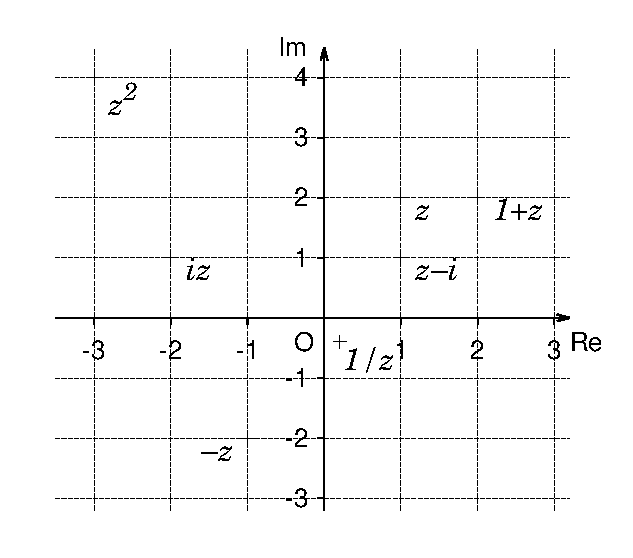
\includegraphics[width=7cm]{cplane1.eps}
    \caption{問\ref{q:univ_comp_plane0}の答え。}\label{fig:cplane1}
\end{figure}

%
\noindent{\textbf{答}}\ref{q:univ_comp_polar0}  
\begin{edaenumerate}<3>
\item \begin{eqnarray*}\sqrt{2}\exp \Bigl(\frac{\pi}{4}\,i\Bigr)\,\,\,\,\,\,\,\,\,\,\,\,\end{eqnarray*}
\item \begin{eqnarray*}2\exp \Bigl(\frac{\pi}{6}\,i\Bigr)\,\,\,\,\,\,\,\end{eqnarray*}
\item \begin{eqnarray*}\exp \Bigl(\frac{3\pi}{2}\,i\Bigr)\,\,\,\,\,\,\,\end{eqnarray*}
\item \begin{eqnarray*}\frac{1}{\sqrt{2}}+\frac{i}{\sqrt{2}}\,\,\,\,\,\,\,\end{eqnarray*}
\item \begin{eqnarray*}-2\,\,\,\,\,\,\,\end{eqnarray*}
\item \begin{eqnarray*}1+\sqrt{3}i\,\,\,\,\,\,\,\end{eqnarray*}
\end{edaenumerate}
\hv

\noindent{\textbf{答}}\ref{q:univ_comp_polar2}  
\begin{edaenumerate}<3>
\item $e^{i7\pi/12}$
\item $e^{-i\pi/12}$
\item $e^{i3\pi/4}$
\item $e^{i\pi/2}$
\item $8e^{i\pi}$
\end{edaenumerate}
\hv

\noindent{\textbf{答}}\ref{q:univ_comp_polar_abs} $z=r_1e^{i\theta_1}$, 
$w=r_2e^{i\theta_2}$とする($r_1, r_2, \theta_1, \theta_2$は実数。$r_1$と$r_2$は0以上)。
\eref{eq:compnum_r}と\eref{eq:comppolar}より, 絶対値と動径は同じである。
従って, $|z|=r_1$, $|w|=r_2$である。
\begin{eqnarray}
zw=r_1e^{i\theta_1}r_2e^{i\theta_2}=r_1r_2e^{i\theta_1}e^{i\theta_2}
=r_1r_2e^{i(\theta_1+\theta_2)}\nonumber\\
\end{eqnarray}
この最後の項を極形式とみれば, その動径は$r_1r_2$である。絶対値と動径は同じなので, 
$|zw|=r_1r_2=|z||w|$, すなわち\eref{eq:abs_zw_absz_absw}が成り立つ。\qed
\hv

%
\noindent{\textbf{答}}\ref{q:univ_comp_polar4}  複素数$z, w$について,
\begin{enumerate}
\item $z=re^{i\theta}$とする。$e^{i\alpha}z=re^{i(\theta+\alpha)}$となる。
これはもとの$z$に対して, 偏角が$\alpha$だけ増えた式
なので, 複素平面上では, 原点を中心に$\alpha$だけ左向きに回転することに対応する。
\hv
\item $z=re^{i\theta}=r\cos\theta+ir\sin\theta$だから,
\begin{eqnarray*}
\overline{z}&=&r\cos\theta-ir\sin\theta\\
&=&r\{\cos(-\theta)+i\sin(-\theta)\}=re^{-i\theta}
\end{eqnarray*}
\end{enumerate}
\hv

\noindent{\textbf{答}}\ref{q:univ_comp_i_pow_i} 
\begin{enumerate}
\item 複素平面に$i$をプロットすると, 動径1, 偏角$\pi/2$であること
は明らかなので, 極形式で表現して$i=e^{\pi i/2}$。
\item 前問の結果の両辺を$i$乗すれば, $i^i=(e^{\pi i/2})^i=e^{\pi i^2/2}=e^{-\pi/2}$。
\item $i^i=e^{-\pi/2}\fallingdotseq e^{-1.5708}\fallingdotseq0.2079$。
\end{enumerate}
\hv

\begin{comment}
%
\noindent{\textbf{答}}\ref{q:univ_comp_polar6} 
\begin{enumerate}
\item $1$
\item $|e^{i\pi/3}-e^{-i\pi/3}|=|2i\sin(\pi/3)|=\sqrt{3}$
\item $|(e^{i\pi/4})^3|=|e^{i\pi/4}|^3=1^3=1$
\item $|e^{i\pi/5} e^{i2\pi/7} e^{i3\pi/11}|=|e^{i\pi/5}||e^{i2\pi/7}||e^{i3\pi/11}|$\\$=1\times1\times1=1$ (このように, $e^{ix}$の形の複素数は, いくつ掛け算しても, 絶対値は1である)
\item 略。
\item 略。
\end{enumerate}
\hv
\end{comment}


% 解答:偏微分
\noindent{\textbf{答}}\ref{q:univ_part_deriv0}  
\begin{eqnarray*}
&&\text{(1) \,\,\,} \frac{\partial f}{\partial x}=2x,\,\,\, \frac{\partial f}{\partial y}=2y\\
&&\text{(2) \,\,\,} \frac{\partial f}{\partial x}=y\exp xy,\,\,\, \frac{\partial f}{\partial y}=x \exp xy\\
&&\text{(3) \,\,\,} \frac{\partial f}{\partial x}=\frac{x}{\sqrt{x^2+y^2}},\,\,\, \frac{\partial f}{\partial y}=\frac{y}{\sqrt{x^2+y^2}}\\
&&\text{(4) \,\,\,} \frac{\partial f}{\partial x}=-\frac{x}{(x^2+y^2)^{3/2}},\,\,\, \frac{\partial f}{\partial y}=-\frac{y}{(x^2+y^2)^{3/2}}
\end{eqnarray*}
\mv

%
\noindent{\textbf{答}}\ref{q:univ_part_deriv2}  $\partial f / \partial x=y\exp(xy)$より, 
\begin{eqnarray*}\frac{\partial}{\partial y}\frac{\partial f}{\partial x}=\exp(xy)+xy\exp(xy)\end{eqnarray*}
また, $\partial f / \partial y=x\exp(xy)$より, 
\begin{eqnarray*}\frac{\partial}{\partial x}\frac{\partial f}{\partial y}=\exp(xy)+xy\exp(xy)\end{eqnarray*}
よって, 
\begin{eqnarray*}\frac{\partial^2 f}{\partial y\partial x}=\frac{\partial^2 f}{\partial x\partial y}=\exp(xy)+xy\exp(xy)\end{eqnarray*}
\mv

\noindent{\textbf{答}}\ref{q:univ_part_deriv4} 
\begin{enumerate}
\item $\partial^2 f/\partial x^2=-(e^y+e^{-y}) \cos x$
\item $\partial^2 f/\partial y^2=(e^y+e^{-y}) \cos x$
\item (1)(2)より明らか。
\end{enumerate}
\mv


% 解答:全微分
\noindent{\textbf{答}}\ref{q:univ_deriv_gas}  
\begin {enumerate}
\item $\rho=P/RT$に値を代入し$\rho=44.08$ mol m$^{-3}$。
\item $\rho=43.96$ mol m$^{-3}$。
\hv
\item それらの差を$d\rho$と書くと, \\
$d\rho=43.96$~mol m$^{-3}-44.08$~mol m$^{-3}=-0.12$~mol~m$^{-3}$。
\item 
\begin{eqnarray*}\frac{\partial \rho}{\partial P}=\frac{1}{RT},\,\,\,\,\,\,\,\, \frac{\partial \rho}{\partial T}=-\frac{P}{RT^2}\end{eqnarray*}
従って, 全微分公式から, 
\begin{eqnarray*}d\rho=\frac{\partial \rho}{\partial P}dP + \frac{\partial \rho}{\partial T}dT
=\frac{1}{RT}dP-\frac{P}{RT^2}dT\end{eqnarray*}
\hv
\item $dT$=1 K, $dP$=1 hPa=$10^2$ Paとして上の式に代入すると, 
$d\rho=-0.12$ mol m$^{-3}$。
\end{enumerate}
\mv

%
\noindent{\textbf{答}}\ref{q:mensekibun01}
\begin{eqnarray*}
\int_{-2}^{2}\Bigl(\int_{0}^{3}(x^2+xy)dx\Bigr)dy
=\int_{-2}^{2}\Bigl[\frac{x^3}{3}+\frac{x^2y}{2}\Bigr]_0^3dy\\
=\int_{-2}^{2}\Bigl(9+\frac{9y}{2}\Bigr)dy
=\Bigl[9y+\frac{9y^2}{4}\Bigr]_{-2}^2
=36
\end{eqnarray*}
\mv

\noindent{\textbf{答}}\ref{q:integ_okashi0} 
位置$(x, y, z)$にある, 体積$dx\,dy\,dz$の直方体の中に
含まれる砂糖の量$dS$は, $C\,dx\,dy\,dz$。これを積分して, 
\begin{eqnarray*}
S=\int_{0}^{c}\int_{0}^{b}\int_{0}^{a}C\,dx\,dy\,dz
\end{eqnarray*}

